\section{Introduction}
\label{sec:intro}
\david{BFT is popular but throughput is difficult to scale.}
Dealing with arbitrary failures is inherently complex; dealing \emph{efficiently} with arbitrary failures even more so. 
Designing correct, scalable BFT~\cite{byzantineGenerals} protocols is thus extremely challenging, and even experts often make mistakes~\cite{zyzzyvaBug, protocolBugsList}.
While one cannot do much about the inherent complexity of BFT, recent work suggests an appealing middle ground.
Instead of creating new, scalable protocols from scratch, one can break down existing (and usually simpler)
% \natacha{and usually simpler?}
protocols into components~\cite{chemistryBehindAgreement} that can be scaled individually~\cite{compartmentalized}.

Gupta et al.~\cite{resilientdb} manually pipelined and partitioned existing BFT protocols, achieving up to $6\times$ throughput improvement.
\sigmodpaper{}~\cite{autocomp} obtained similar results with simple, local, \emph{program rewrites} for Paxos~\cite{paxosComplex}: \textbf{decoupling} (splitting logic across nodes) and \textbf{partitioning} (splitting data across nodes), as seen in \Cref{fig:rewrites}.
Their rewrites are promising because they are protocol-agnostic and rule-driven: given a protocol written in a distributed DSL~\cite{dedalus}, the rewrites can be used to correctly modify any protocol.
However, these rewrites were proven correct assuming non-Byzantine failures only.

This paper modifies the rewrites introduced by \sigmodpaper{} and proves the correctness of the resulting rewrites when applied to BFT protocols.
% In this paper we investigate the vulnerability of these rewrites to Byzantine attacks, and we enhance the rewrites to provably tolerate Byzantine behavior.
% \jmh{Rather than end on a negative note, end on a plan: "HOwever, these rewrites were proven correct assuming non-Byzantine failures; this weakness makes the rewrites unsafe for optimizing BFT protocols. In this paper we investigate the vulnerability of these rewrites to Byzantine attacks, and we enhance the rewrites to provably tolerate Byzantine behavior. [Paragraph Break] To illustrate the vulnerabilities of the rewrites in Chu et al., consider..." Then you can delete the short paragraph after this one.}
% \david{Joe: State that it would be good to apply them to BFT. Emphasize that it's our hypothesis. Natacha: Cite Suyash's work on ResilientDB breaking down protocols into components}
% \natacha{Maybe Suyash's work fits better here. I would love to see a sentence here that talks about the potential win. "This is a missed opportunity. Gupta et al. shows that with careful engineering, pipelining, etc. BFT protocols can be made up to Xxx faster without any algorithmic changes}

% \david{Provide example of unintuitive new vector of attack: partitioning}
% To illustrate the challenge, consider a simple vote-counting protocol that stores votes in a set.
% It exposes two APIs: \texttt{appendVote(id)} and \texttt{count()}.
% The \texttt{appendVote(id)} function verifies each vote before inserting it into the set.
% The \texttt{count()} function hash partitions votes by id, counts the number of votes in each partition, then sums up the counts across partitions.
% Because votes with different ids are independent, \sigmodpaper{}'s rewrites assert that this set as a whole can be partitioned and distributed across nodes.

% Let us assume that this set is BFT, but Byzantine nodes can interact with it via API calls.
% In the presence of Byzantine failures, partitioning would be \emph{unsafe}.
% A Byzantine node could send the same, valid, vote to multiple nodes, inflating the final count.
% Because the partitioning rewrite was not designed to handle Byzantine failures, individual nodes do not verify whether the partitioning invariant is violated \nc{They do, just not the same invariant as in the CFT?} and become vulnerable to duplication attacks.
% In general, without modifications, the rewrites presented by \sigmodpaper{} are unsafe when applied to BFT protocols.
% \david{Natacha: Make clear that we need to modify the partitioning rewrites, not the invariants. Make clear what would have happened before partitioning (votes cannot be inserted multiple times). Think about BFT example where this would be a problem where the original protocol was completely BFT? Would be nice if example was PBFT. Example: decoupling, 1 original node sending its prePrepare to the committer. Can send different command; the committer doesn't re-check that the digest matches the command.
% Joe: Another possibility: don't give full self-contained example. Just say what could go wrong with decoupling and partitioning.}

\begin{figure}[t]
    \centering
    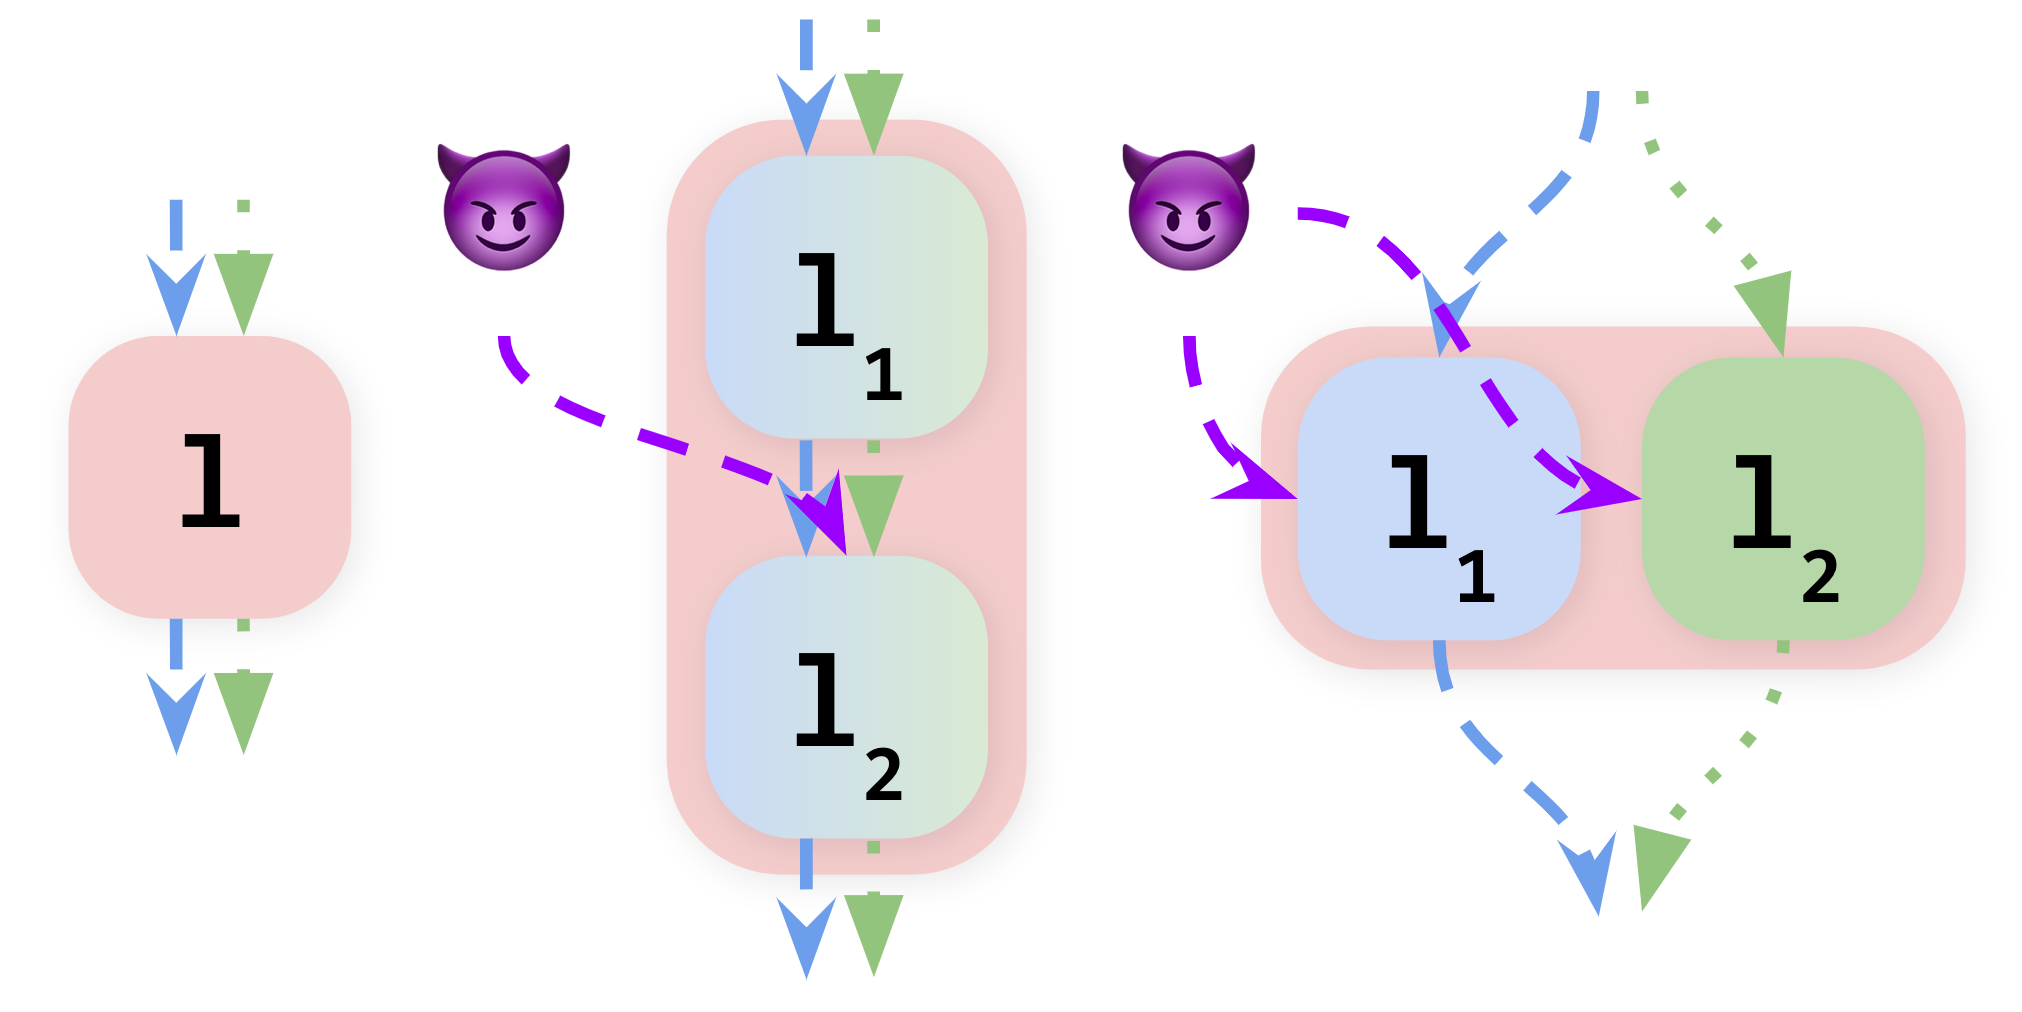
\includegraphics[width=0.8\linewidth]{assets/rewrites.png}
    \caption{Decoupling (middle) and partitioning (right), splitting a node $l$ into two nodes $l_1$ and $l_2$. Byzantine nodes (evil emoji) can insert messages on decoupled message channels and duplicate messages across partitions.}
    \label{fig:rewrites}
\end{figure}


\david{Example of vector of attack: decoupling on PBFT.}
To illustrate the challenge, consider the critical path of PBFT~\cite{pbft}, a fundamental BFT protocol that reaches consensus across $3f+1$ replicas.
Replicas in PBFT receive \textsc{PrePrepare} messages from a primary replica: these messages contain, among other things, a command to execute, its hash digest, and a signature from the primary over the hash digest.
The replica accepts the message if the digest is indeed the hash of the command and the signature is valid.
In a later phase, once this replica receives $2f+1$ \textsc{Commit} messages (which also contain a digest) from other replicas, it will compare the digest within the \textsc{Commit}s to the digest of the \textsc{PrePrepare} it received earlier; if the digests match, then the replica will execute the command.

Because the replica monotonically accumulates sets of \textsc{PrePrepare} and \textsc{Commit} messages through time, the rewrites from \sigmodpaper{} suggest that replicas can be scaled up via monotonic decoupling.
% \tyler{For a single node,} 
For each node, the logic that collects \textsc{PrePrepare} messages and the logic that collects \textsc{Commit} messages can be decoupled into two nodes: a \emph{pre-preparer} and \emph{committer} \jmh{reference Figure 1 here to illustrate. I recommend you change it to Fig 1a and 1b, one each for decoupling and partitioning, so that here you can reference "$l_1$ and $l_2$ of Figure 1a", rather than "$l_1$ and $l_2$ of the middle of Figure 1"?}.
% \tyler{two nodes, a pre-prepreparer and committer, where the pre-preparer forwards \textsc{PrePrepares} to its own committer, which later compares digests and executes the command.} 
Crucially, each pre-preparer \jmh{(e.g. $l_1$)} must forward \textsc{PrePrepare}s to its own committer \jmh{($l_2$)}so it can later compare digests and execute the command.
The remaining phases of PBFT can be similarly decoupled, as we will discuss in detail in \Cref{sec:eval}.

% \tyler{Intuitively, decoupling logic into two nodes increases the parallelism and therefore the throughput of the system. However,}
Intuitively, decoupling logic into two nodes reduces load on any one machine and can improve throughput.
However, in the presence of Byzantine failures, this decoupling would be \emph{unsafe}.
A single Byzantine node could \jmh{masquerade as two pre-preparers, and} send two committers doctored \textsc{PrePrepare}s with the same digest but different commands.
Committers, without checking whether the message was forwarded from their own pre-preparers, would then execute the wrong commands, breaking the consensus invariant.
Because \sigmodpaper{}'s decoupling rewrite was not designed to handle Byzantine attacks, the messages between decoupled nodes are neither signed nor verified, allowing Byzantine nodes to insert their own messages as seen in \Cref{fig:rewrites}.


% \natacha{What is the flow you were going for for the next 3/4 paragraphs? It's hard to follow the order. }
% \natacha{Is it the rewrites that are different, the conditions on which you can apply them, or just the proofs? You switch between all of them and it's a bit confusing.}
% \natacha{I'd shorten the next paragraph to be more direct. We first address two challenges, etc. First, we must precisely model all possible Byz behaviour in the system. If the non-scaled protocol is correct in a world in which all Byz behaviour is possible, the scaled protocol should also be correct. Byz nodes can execute arbitrary program logic and send arbitrary messages .. }

% \david{Why rewrites are vulnerable and how we modify them.}
% \natacha{Would be nicer to talk in terms of challenges and solutions? What are he two/three challenges you had to address, and then describe how your solution addresses those. I would say there are two challenges 1) how to actually model correctness (for this you need to express all possible Byz behaviour}
% We modify the rewrites by hardening message channels introduced by decoupling and partitioning against Byzantine attacks.
% Decoupling converts dataflow within a single-node process into message channels between nodes, which Byzantine nodes can populate with arbitrary messages. We modify decoupling such that messages on these channels are signed and verified.
% \natacha{Why do you need signatures rather than MACs?}\heidi{Transferability?}
% Partitioning splits messages across nodes; Byzantine nodes can send messages to incorrect partitions.
% We modify partitioning such that nodes check whether the message they receive belongs to their partition.
% \david{How we prove correctness.}
% In order to prove the correctness of our modified rewrites, we will demonstrate the following:
% (1) Byzantine nodes can be modeled \jmh{by a "randomization construction" or some such name} \emph{entirely based on the output they produce},
% (2) Byzantine nodes in a protocol that has been rewritten are no more powerful than Byzantine nodes in the original protocol, and
% (3) Message channels introduced or modified by the rewrites are safe against Byzantine nodes.

% \david{Heidi: Introduce rewrites.}
\david{Our rewrites.}
To prevent the attack above, we will modify decoupling with \emph{sender verification} (\Cref{sec:sender-verification}), which signs and verifies each message sent between decoupled nodes.
We will also modify partitioning with \emph{message verification} (\Cref{sec:message-verification}), such that each partition individually verifies that it is receiving the correct subset of hash-partitioned messages.

\david{Our proof strategy.}
% \jmh{Given an input protocol that is BFT...?}
Given an input protocol that is BFT, our proof strategy is two-fold: we show that (1) to nodes untouched by the rewrites, Byzantine nodes in the rewritten protocol cannot generate any more messages than they could have generated before, and
\david{Natacha: Change all instances of ``compare Byzantine behavior'' or power to discussion on how Byzantine nodes can't send more things that they could have sent before.}
(2) for modified nodes, all invariants required by the rewrites are reinforced against Byzantine attacks.
With these guarantees, any Byzantine attacks on the untouched nodes in the rewritten protocol would be identical to a Byzantine attack in original protocol (which is already BFT), and any Byzantine attacks on the modified nodes are ineffective.

\david{Modeling Byzantine behavior.}
In order to discuss what messages a Byzantine node can produce, we must formally model \emph{all} possible Byzantine behavior as part of our proof framework.
This is tricky: Byzantine behavior is, by definition, arbitrary.
% , with the caveat that one cannot break standard cryptographic primitives.
To this effect, we make the following observations: (1) a Byzantine node's behavior is a function of its outputs, and (2) the set of all possible Byzantine behaviors is 
% \jmh{eventually executed by nodes that execute random behaviors?} 
exactly the set of all \emph{random} behaviors.
% \tyler{Do you need to emphasize randomness to prove correctness? My worry is that randomness might suggest to a reader that you might empirically evaluate your correctness with e.g. fuzzing as opposed to a formal proof. The proof-of-correctness in section 5 does not seem to require randomness at least to my understanding.}
We introduce the \emph{\randomSimulator{}}\footnote{Jorge Luis Borges' story \textit{The Library of Babel} posits a library of books composed of every possible ordering of characters. By definition, this library contains all books, though it may take arbitrary time to find good ones.}, a theoretical gadget that simulates all possible Byzantine behavior in a protocol-agnostic way through randomness.
At any point in time, the \randomSimulator{} can generate arbitrarily many random messages to all input channels.
This theoretical gadget allows us to compare Byzantine behaviors and prove the correctness of the modified rewrites.

% \natacha{The bullet structure is a bit strange -> (3) is the end goal and (2)/(1) are necessary steps to achieve 3. Putting them as the same "level" is confusing. I would rephrase as follows: }
% \natacha{The key challenge in proving correctness in a BFT setting stems from having to model *all* possible Byzantine behavior as part of our proof framework, before showing that the set of behaviour post rewrites is a strict subset of allowable behaviour in the original protocol. Byzantine behaviour is, by definition, arbitrary. Nodes cannot break standard cryptographic primitives but can otherwise behave in arbitrary ways.  To this effect, we introduce the Borgesian simulator, a gadget that simulates all possible Byzantine behaviour in an protocol agnostic way by allowing Byzantine nodes to behave randomly. At any given point in time, the Borgesian gadget can generate infinitely many random messages to all input channels}


% The power of \randomSimulator{}s can be compared on the cryptographic keys they have access to, the signed messages they have received, and the input channels they can send to. \natacha{I can't understand this sentence}
% We will show that our rewrites do not allow Byzantine nodes access to more keys \natacha{What does it means for nodes tohave additional keys?} additional messages that they can receive are useless, and that the new and modified input channels are resilient against Byzantine messages. \jmh{This last sentence is not apropos to the topic sentence of the paragraph. Maybe doesn't belong in this paragraph?}

\david{Results.}
Our initial results are promising.
The modified rewrites are simple to check, yet applying them scales the throughput of PBFT by $5\times$ when applied to its critical path.
% \david{Should we end this paragraph with some implications of the larger picture?}

% The difference in the proofs used by this paper and \sigmodpaper{} can be boiled down to the difference in what messages a correct machine can receive.
% \sigmodpaper{} made two implicit assumptions in their rewrites that do not hold in a Byzantine environment:
% (1) New machines will execute program logic as intended, and
% (2) Modified input channels will be populated with the expected messages.

% The first assumption is violated if a new machine becomes Byzantine. \heidi{there was a switch here from nodes to machines, i prefer nodes}
% We will show that new Byzantine machines are no more powerful than Byzantine machines in the original protocol.
% \chris{"...no more powerful than old Byzantine machines that existed before protocol rewrites"?}
% In order to prove this property, we must carefully define what messages Byzantine machines are capable of sending.

% The second assumption is violated if Byzantine machines attempt to violate the modified input channels' invariants, as in the partitioning example presented earlier. \nc{Not sure I get that}
% \jmh{Note that in the set-of-votes example above, the invariant is explicit: to ensure local duplicate detection works, input channel must obey partitioning.}
% We will modify the rewrites such that nodes detect and discard any invariant-violating messages.